\providecommand\forslides{1}

 
%%%%%%%%%%%%%%%%%%%%%%%%%%%%%%%%%%%%%%%%%%%%%%%%%%%%%%%%%%%%%%%%%%%%%%%%%%%%%

\ifnum\forslides=1

  \documentclass{beamer}
  \usepackage{etex}
  \reserveinserts{108}
  \usepackage{animate}
  \renewcommand{\cite}[1]{[Ref in notes]}

\else

  \documentclass[11pt,a4paper,twoside]{report}
  %%%%%%%%%%%%%%%%%%%%%%%%%%%%%%%%%%%%%%%%%%%%%%%%%%%%%%%%%%%%%%%%%%%%%%%%%%%%%
  \usepackage{beamerarticle}
  \usepackage{graphicx}
  \setlength{\parindent}{0in}
  %%%%%%%%%%%%%%%%%%%%%%%%%%%%%%%%%%%%%%%%%%%%%%%%%%%%%%%%%%%%%%%%%%%%%%%%%%%%%
  \renewcommand{\lecture}[2]{\chapter{#1}}
  %%%%%%%%%%%%%%%%%%%%%%%%%%%%%%%%%%%%%%%%%%%%%%%%%%%%%%%%%%%%%%%%%%%%%%%%%%%%%
  \newcommand\NormalArticleFrameTitleMode{%
    \renewcommand{\frametitle}[1]{%
      \marginpar{\raggedright ##1 (\insertframenumber)}%
    }%
  }
  \newcommand\ExercisesArticleFrameTitleMode{
    \renewcommand{\frametitle}[1]{%
      ##1%
    }%
  }
  \NormalArticleFrameTitleMode
  %%%%%%%%%%%%%%%%%%%%%%%%%%%%%%%%%%%%%%%%%%%%%%%%%%%%%%%%%%%%%%%%%%%%%%%%%%%%%
  \renewcommand{\familydefault}{\sfdefault}
  
  %%%%%%%%%%%%%%%%%%%%%%%%%%%%%%%%%%%%%%%%%%%%%%%%%%%%%%%%%%%%%%%%%%%%%%%%%%%%%

\fi

\usepackage{subfigure,amsmath}
\usepackage{float}
\usepackage{subfigure}
\usepackage{verbatim}
% %\usepackage[xindy]{glossaries}
% \usepackage{enumitem}
\usepackage{tikz}
\usepackage{verbatim}
\usepackage{xcolor,colortbl}
\usepackage{acronym}
\usepackage{hyperref}

\acrodef{ML}{Machine Learning}
\acrodef{HCI}{Human-Computer Interaction}
\acrodef{GP}{Gaussian Process}
\acrodef{MVG}{Multi-Variate Gaussian}
\acrodef{SLM}{Statistical Language Model}
\newcounter{taskcounter}

\definecolor{highlightcol}{rgb}{1,0.184,0.275}
\newcommand{\focus}[1]{{\textcolor{highlightcol}{\bf #1}}}
\newcommand{\up}[1]{{\textcolor{red}{\bf #1}}}
\newcommand{\down}[1]{{\textcolor{OliveGreen}{\bf #1}}}
\definecolor{yellowhighlighter}{rgb}{1,0.984,0.8}
\definecolor{nicered}{rgb}{1,0,0}
\definecolor{niceorange}{rgb}{1,0.6,0}
\newcommand{\highlightred}[1]{{\textcolor{nicered}{\bf #1}}}
\newcommand{\highlightorange}[1]{{\textcolor{niceorange}{\bf #1}}}
\newcommand{\todo}[1]{{\textcolor{green}{\bf TODO: #1}}}

\newcommand{\bX}{\mathbf{X}}
\newcommand{\bx}{\mathbf{x}}
\newcommand{\bPars}{\boldsymbol\Theta}
\newcommand{\by}{\mathbf{y}}
\newcommand{\blf}{\mathbf{f}}

\graphicspath{{../Code/GP/}{Figures/}}

\newsavebox{\selvestebox}
\newenvironment{task}
  {\stepcounter{taskcounter}
  \newcommand\colboxcolor{F87A17}%
   \begin{lrbox}{\selvestebox}%
   \begin{minipage}[t]{0.15\textwidth}%\dimexpr\columnwidth-2\fboxsep\relax}
   \textbf{TASK [\arabic{taskcounter}]}%
   \end{minipage}%
   \begin{minipage}[t]{0.8\textwidth}%
   }
%   \begin{minipage}[t]{.45\textwidth}
%  Basic Problems of Single-Photon Polymerization:
%  \begin{itemize}
%  \item layer-by-layer type of manufacturing (limits possible geometries)
%  \item suppression through undesired quenching of radicals
%  \item diffraction limits
%  \end{itemize}
% \end{minipage}
  {\end{minipage}\end{lrbox}%
   \begin{center}
   \fcolorbox[HTML]{\colboxcolor}{FFCC99}{\usebox{\selvestebox}}
   \end{center}}

\newcommand{\LectureTitlePage}{%
    % \setcounter{framenumber}{0}
    \global\def\inserttitle{{Lecture \insertlecturenumber: \insertlecture}}
    \global\def\insertshorttitle{{Lecture \insertlecturenumber: \insertlecture}}
    % \global\def\insertdate{\lecturedate}
    % \global\def\insertshortdate{\lecturedate}
  \titlepage
}

\AtBeginLecture{
    \begin{frame}[plain]
      \LectureTitlePage
    \end{frame}
}
\setbeamertemplate{caption}[numbered]

\title{Non-parametric Bayesian Methods in Machine Learning}
\author{Dr. Simon Rogers\\School of Computing Science\\University of Glasgow\\simon.rogers@glasgow.ac.uk\\@sdrogers}

%\includeonlylecture{Touchscreen}


\begin{document}

\mode<all>

\begin{frame}
	\titlepage
\end{frame}

\mode<all>

%% Outline.tex
\begin{frame}
	\frametitle{Outline}
	\begin{itemize}
		\item {\bf FIX ME AT THE END}
		\item (My) Bayesian philosophy
		\item Gaussian Processes for Regression and Classification
		\begin{itemize}
			\item GP preliminaries
			\item Classification (including semi-supervised)
			\item Regression application 1: clinical (dis)-agreement
			\item Regressopn application 2: typing on touch-screens
		\end{itemize}
		\item Dirichlet Process flavoured Cluster Models
		\begin{itemize}
			\item DP preliminaries
			\item Idenfitying metabolites
			\item (if time) Cluster models for multiple data views
		\end{itemize}
	\end{itemize}
\end{frame}

\begin{frame}
	\frametitle{About me}
	\begin{itemize}
		\item I'm not a statistican by training (don't ask me to prove anything!).
		\item Education:
		\begin{itemize}
			\item Undergraduate Degree: Electrical and Electronic Engineering (Bristol)
			\item PhD: Machine Learning Techniques for Microarray Analysis (Bristol)
		\end{itemize}
		\item Currently:
		\begin{itemize}
			\item Lecturer: Computing Science
			\item Research Interests: Machine Learning and Applied Statistics in Computational Biology and \ac{HCI}
		\end{itemize}
	\end{itemize}
	
\end{frame}

\mode<all>

%% Bayesian intro
\lecture{Bayesian Inference}{bayes}

\begin{frame}
	\frametitle{Bayesian Inference}
	Standard setup:
	\begin{itemize}
		\item We have some data $\bX = \{\bx_1,\ldots,\bx_N\}$
		\item We have a model $p(\bX|\bPars)$
		\item We define a prior $p(\bPars)$
		\visible<2->{
			\item We use Bayes rule (and typically lots of computation) to compute (or estimate) the posterior:
			\[
				p(\bPars|\bX) = \frac{p(\bX|\bPars)p(\bPars)}{p(\bX)}
			\]
		}
	\end{itemize}
\end{frame}

\begin{frame}
	\frametitle{Why Be Bayesian?}
	\begin{itemize}
		\item<2->Ability to incoroporate prior information?
		\item<3->Ability to compute posterior densities (combine prior with likelihood)?
		\item<4->Ability to compare models via marginal likelihood?
		\item<5->For me: the ability to integrate out model parameters completely\ldots
	\end{itemize}
\end{frame}


\begin{frame}
	\frametitle{Why be Bayesian?}
	\begin{itemize}
		\item We're often not interested in parameter values
		\item We're normally interested in something that is a function of the parameter values e.g.:
		\begin{itemize}
			\item Within \ac{ML} we are often interested in making predictions (predicing $y_*$ from $\bx_*$).
			\item This will often require values of some parameters $\bPars$
			\item Being Bayesian allows us to \emph{average} over uncertainity in parameters when making predictions:
			\[
				p(y_*|\bx_*,\bX) = \int p(y_*|\bx_*,\bPars)p(\bPars|\bX)~d\bPars
			\]		
		\end{itemize}
		\item This for me, is the biggest Bayesian selling point!
	\end{itemize}
\end{frame}

\mode<all>

\input{GPIntro}

\mode<all>
% CHI keyboard work

\lecture{Application: Touchscreen typing}{Touchscreen}

\begin{frame}
	\frametitle{Typing on touchscreens}
	\begin{itemize}
		\item Most people have smartphones
		\item Most smartphones have touchscreens
		\item Touchscreens are small
		\item Keyboards on touchscreens are small
		\item Typing on them is hard!
		\begin{itemize}
			\item \ldots but people type on them a lot
		\end{itemize}
	\end{itemize}
\end{frame}

\begin{frame}
	\frametitle{Background 1: Why is it hard?}
	\begin{itemize}
		\item Occlusion of target by finger
		\item `fat finger' problem
		\item Small targets
		\item Demo: \url{http://bit.ly/1nBws97}
		\visible<2->{
			\item Quite a bit of work in this area:
			\begin{itemize}
				\item Holz and Baudisch
				\item Henze (100,000,000 taps)
			\end{itemize}
			\item Collecting data is fairly easy
			}
	\end{itemize}
\end{frame}

\begin{frame}
	\frametitle{Background 2: All users are different}
	\begin{figure}[tbh]
		\centering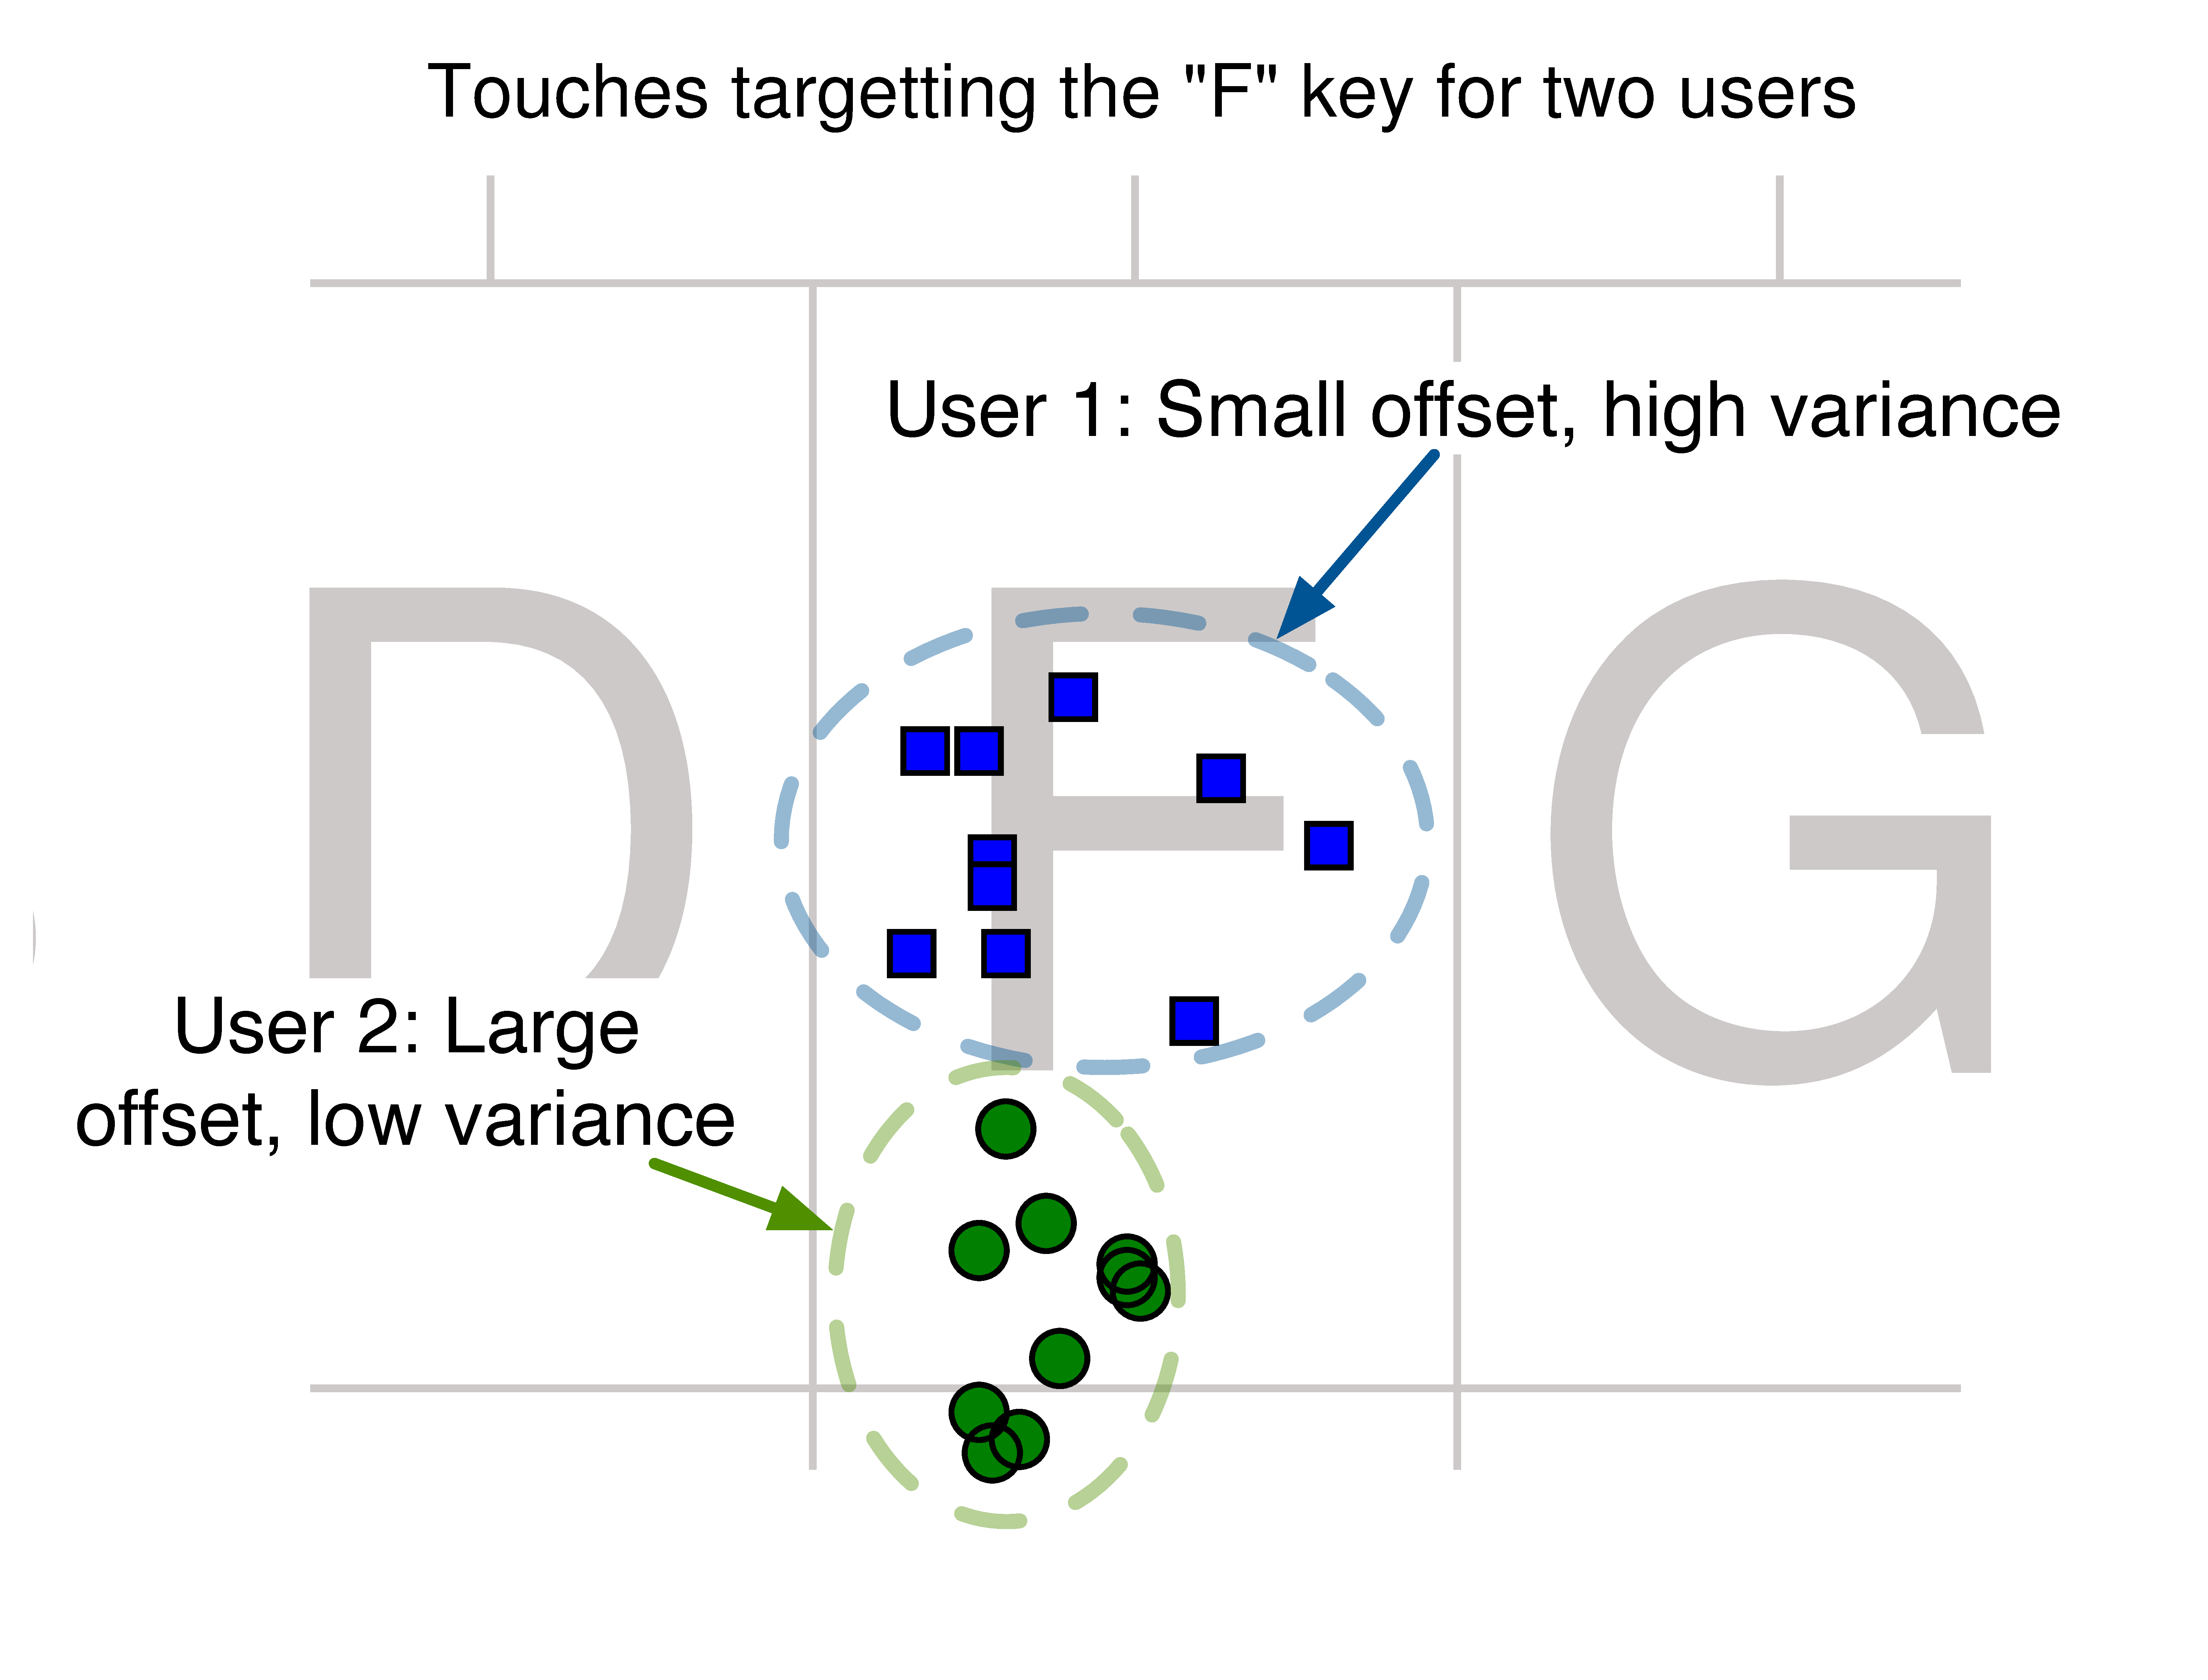
\includegraphics[width=0.8\linewidth]{two_users_annotated.pdf}
		\centering\caption{\label{fig:two_users_annotated}Touches recorded by two users aiming for the `F' key. User 2 has high bias and low variance, user 1 has low bias and high variance.}
	\end{figure}
\end{frame}

\begin{frame}
	\frametitle{Background 3: Current systems (maybe?)}
	\begin{itemize}
		\item Touch is boxed into nearest key.
		\item Key ID is passed to a \ac{SLM}.
		\item \ac{SLM} is made up of probabilities of observing certain character strings (from large text corpora).
		\item \ac{SLM} can swap characters to make the character string more likely.
		\begin{itemize}
			\item e.g. `HELLP $\rightarrow$ HELLO'
		\end{itemize}
	\end{itemize}
\end{frame}


\begin{frame}
	\frametitle{Our idea}
	\begin{itemize}
		\item There is a lot of uncertainty present in touch (bias and variance)
		\item Boxing a touch into a key is probably bad
		\item Why can't we pass a \emph{distribution} to the \ac{SLM}?
		\begin{itemize}
			\item Pass the uncertainty onwards
			\item Being Bayesian!
		\end{itemize}
		\visible<2->{
			\item Can use a user specific GP regression model to predict target from input touch.
		}
	\end{itemize}
\end{frame}

\begin{frame}
	\frametitle{The model}
	\begin{itemize}
		\item We use independent GP regressions for predicting $x$ and $y$ offsets.
		\item Training data:
		\begin{itemize}
			\item Each user typed phrases provided to them.
			\item Data: the $x,y$ location of the recorded touch (i.e. $\bx_n = [x_n,y_n]^T$). Target: the center of the intended key minus the touch (i.e. the offset).
		\end{itemize}
		\item<2-> Used a \ac{GP} with zero mean and a composite covariance:
		\[
			C(\bx_1,\bx_2) = a \bx_1^T\bx_2 + (1-a)\exp \{ -\gamma || \bx_1 - \bx_2 ||^2 \}
		\]
	\end{itemize}
\end{frame}

\begin{frame}
	\frametitle{The model}
	\centering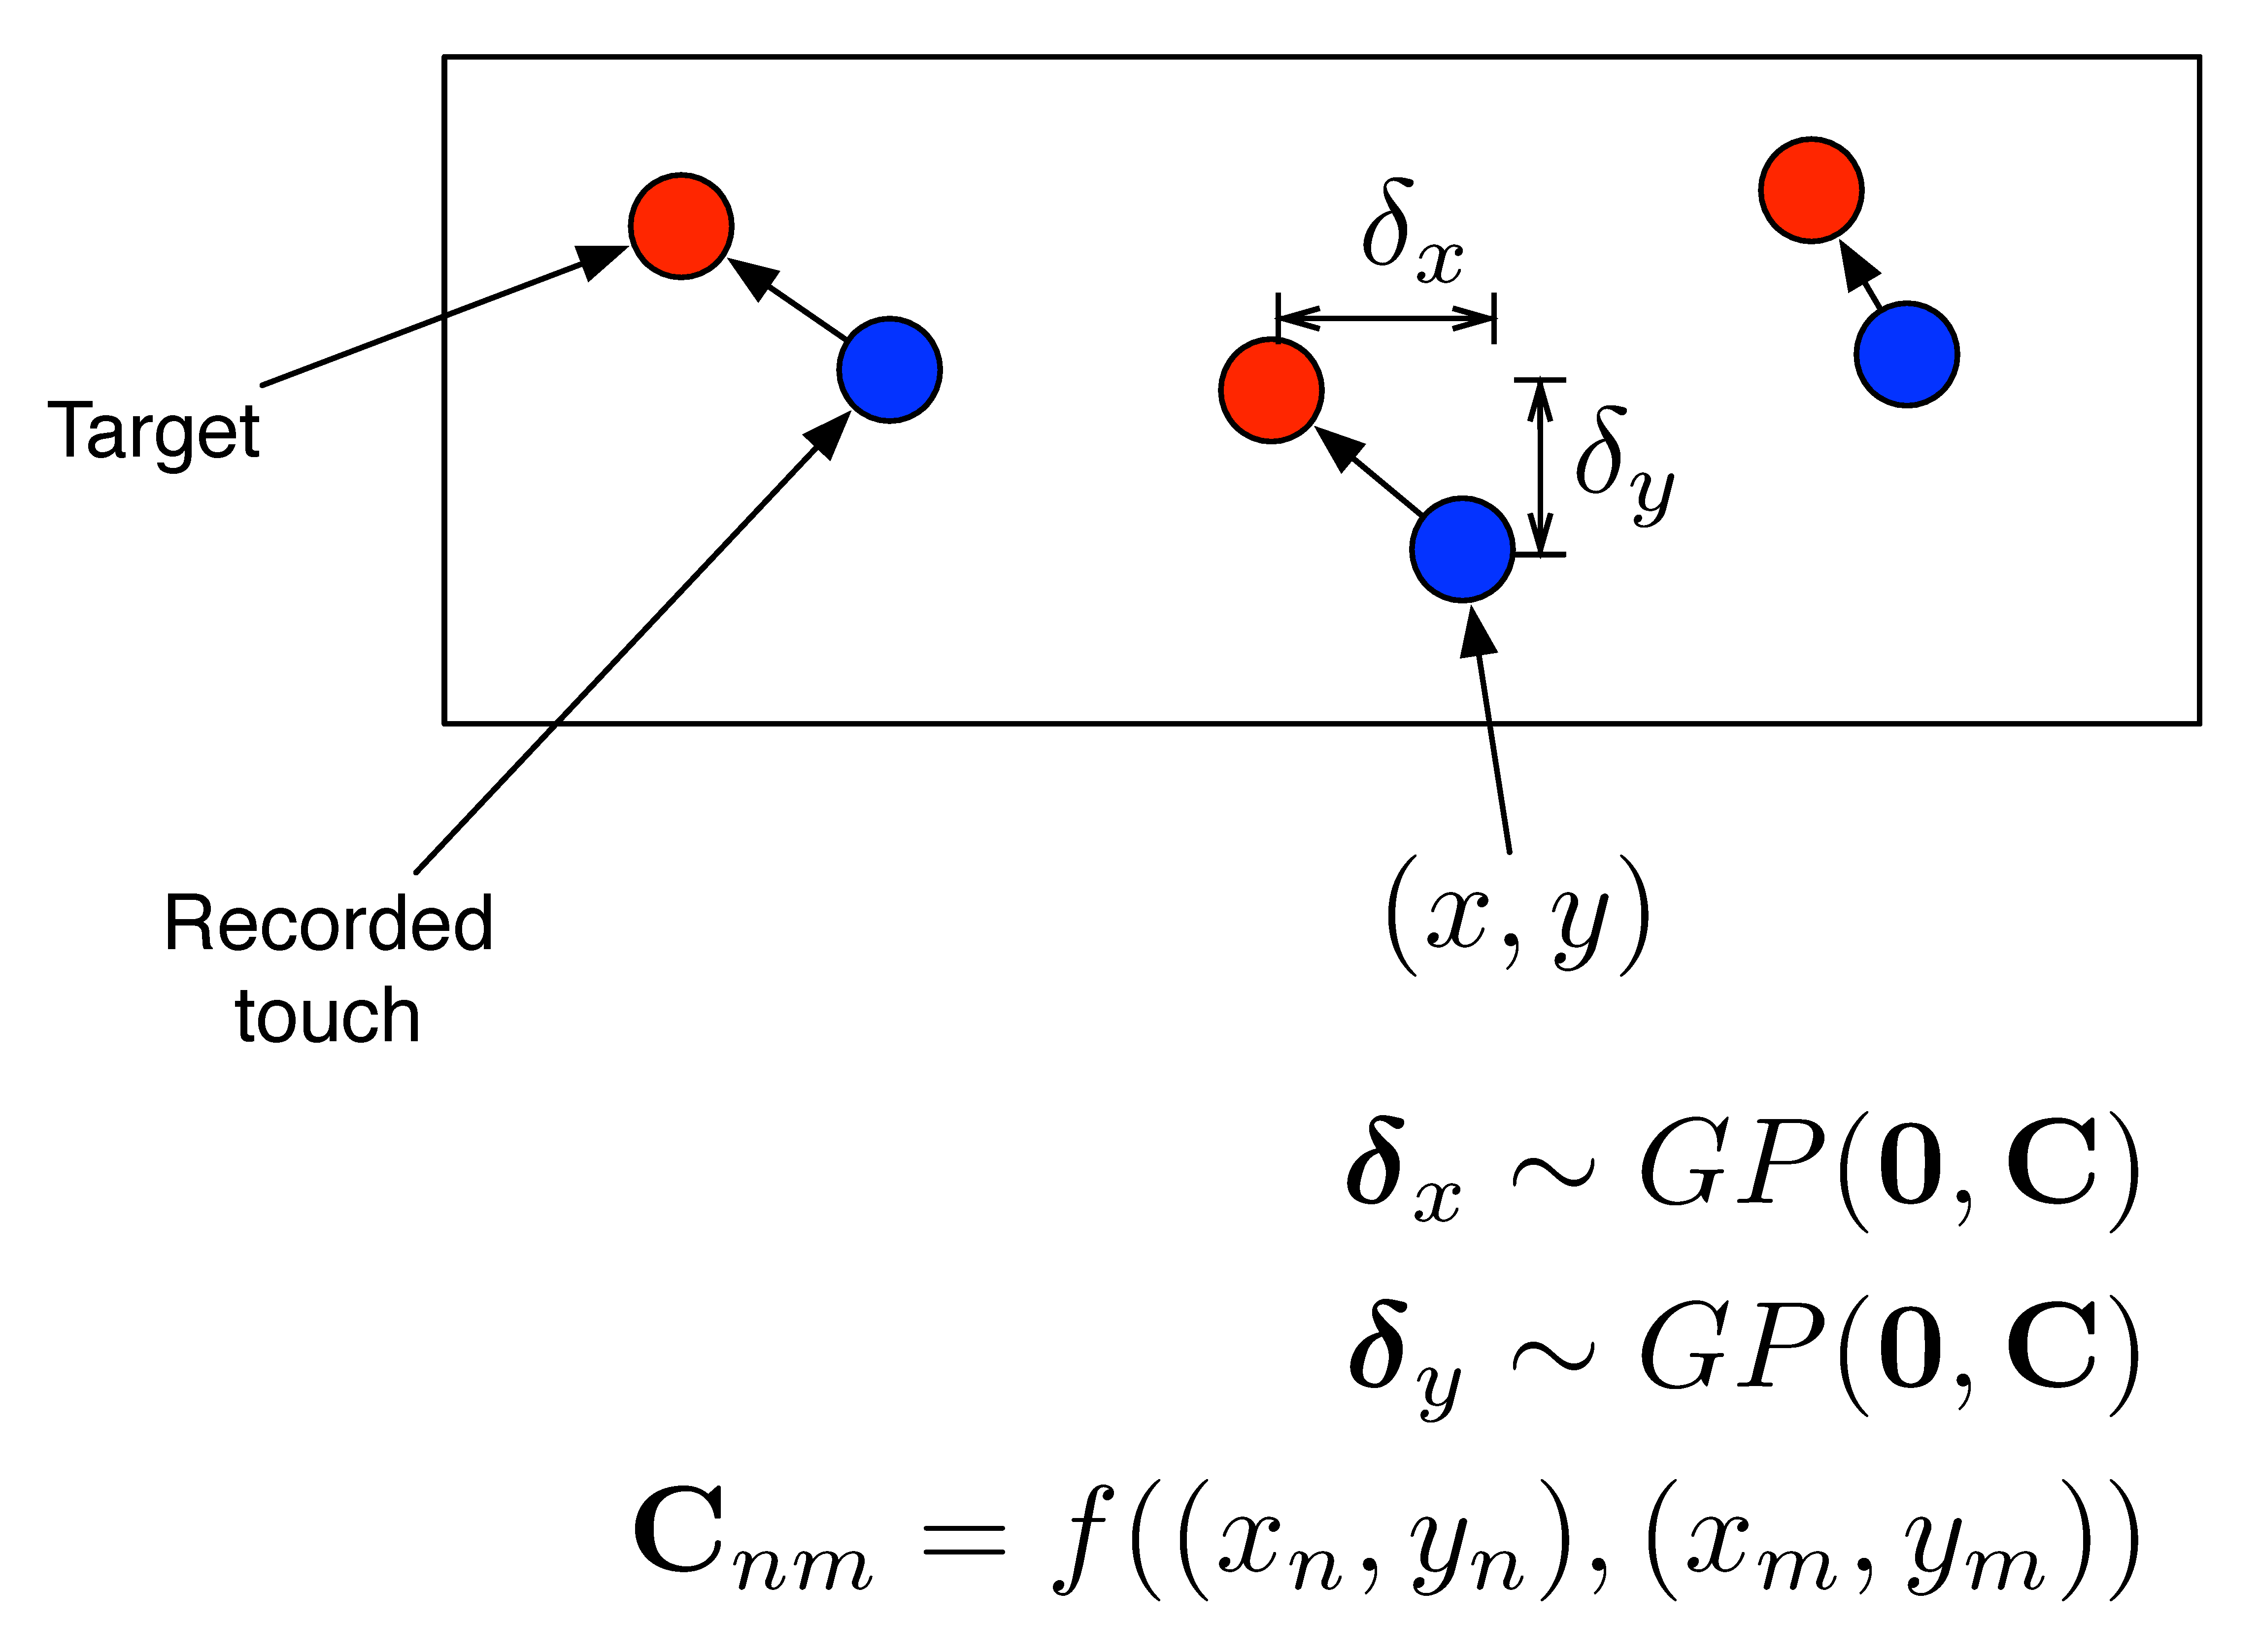
\includegraphics[width=0.7\linewidth]{touchmodel}
	\begin{itemize}
		\item $x$ and $y$ offsets both depend on $x$ and $y$ position of touch
		\item Have also used raw capacitive sensor data as input
		\begin{itemize}
			\item Potentially better (more info) but only accessible on some devices
		\end{itemize}
	\end{itemize}
\end{frame}


\begin{frame}
	\frametitle{System cartoon}
	\begin{figure}
		\centering\includegraphics<1>[width=0.8\linewidth]{cartoon1.pdf}
		\centering\includegraphics<2>[width=0.8\linewidth]{cartoon2.pdf}
		\centering\includegraphics<3>[width=0.8\linewidth]{cartoon3.pdf}
		\centering\includegraphics<4>[width=0.8\linewidth]{cartoon4.pdf}
		\centering\caption{Train GPs to predict the intended touch from an input touch. The flexibility of GPs means that the mean and covariance of the offset can vary across the keyboard.}
	\end{figure}
\end{frame}

\begin{frame}
	\frametitle{System cartoon}
	\begin{figure}[tbh]
		\centering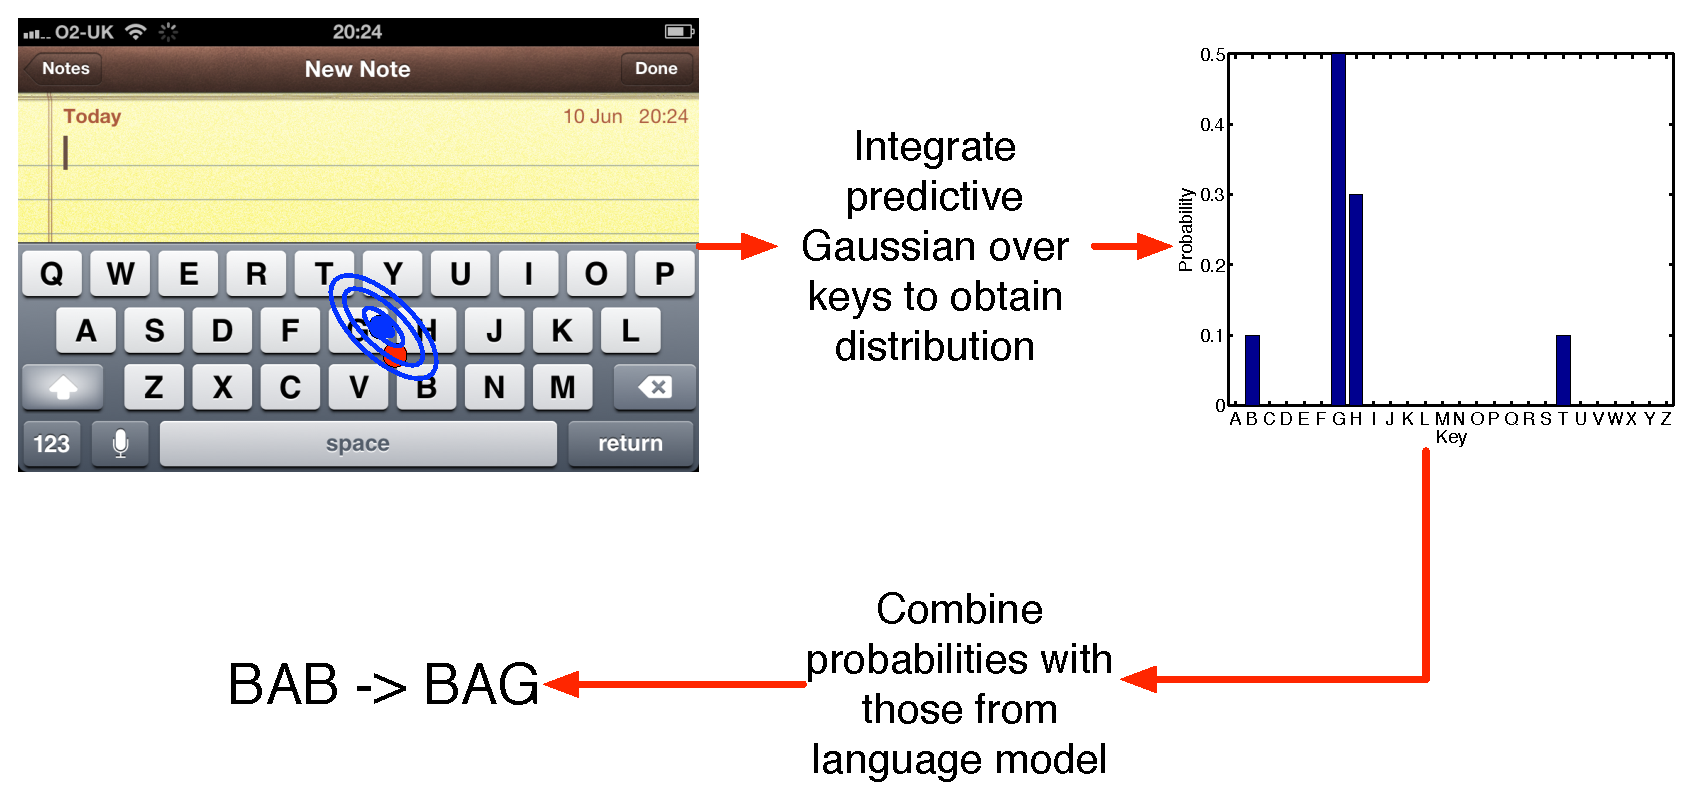
\includegraphics[width=\linewidth]{touchcartoon.pdf}
		\centering\caption{\label{fig:touchcartoon}The complete system}
	\end{figure}
\end{frame}


\begin{frame}
	\frametitle{Video}
	\begin{itemize}
		\item \url{http://www.youtube.com/watch?v=llQI5gV5l74}
	\end{itemize}
\end{frame}

\begin{frame}
	\frametitle{The experiment}
	\begin{itemize}
		\item 10 participants
		\item Calibration data collected for each
		\begin{itemize}
			\item Note: calibration task matters
		\end{itemize}
		\item each did $3\times$ 45 minute sessions, typing whilst sitting, standing and walking. [more details in paper]
		\item Compared:
		\begin{itemize}
			\item GPtype (our system), Swiftkey (commercial Android keyboard), GP only (just offset, no \ac{SLM}), baseline (boxing, no \ac{SLM}).
		\end{itemize}
	\end{itemize}
\end{frame}

\begin{frame}
	\frametitle{Results}
	\begin{figure}[tbh]
		\centering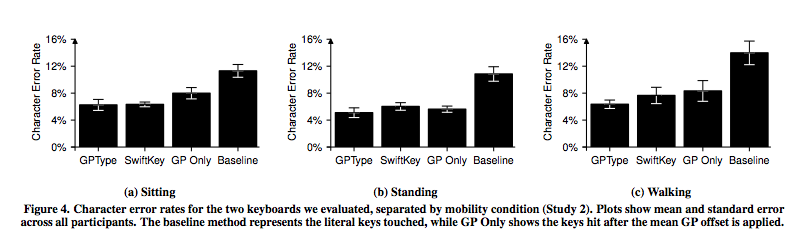
\includegraphics[width=1.0\linewidth]{gptype_results.png}
		\centering\caption{\label{fig:gptype_results}Results of GPType experiment}
	\end{figure}
	\begin{itemize}
		\item GPType marginally (stat sig) better than Swiftkey.
		\begin{itemize}
			\item A {\bf lot} of people work on SwiftKey
		\end{itemize}
		\item Baseline awful!
	\end{itemize}
\end{frame}

\begin{frame}
	\frametitle{Explicit uncertainity control}
	\begin{itemize}
		\item In GPType, uncertainity is handled implicitly
		\item As user typing becomes more uncertain, more power given to language model
		\item Could users \emph{explicitly} control this?
		\begin{itemize}
			\item Certain inputs: no \ac{SLM} control (slang, names, etc)
			\item Uncertain inputs: high \ac{SLM} control
		\end{itemize}
		\item Use pressure to control certainty:
		\begin{itemize}
			\item High pressure: high certainty
			\item Low pressure: low certainty
		\end{itemize}
	\end{itemize}
\end{frame}

\begin{frame}
	\frametitle{Do users know when \ac{SLM} will fail?}
	\centering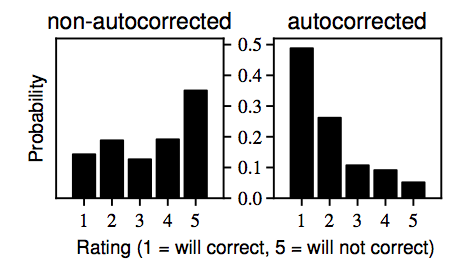
\includegraphics[width=\linewidth]{autocorrect}
	\begin{itemize}
		\item Users given phrases and asked whether they thought autocorrect would change them incorrectly
		\item Users quite good at understanding \ac{SLM} failings
	\end{itemize}
\end{frame}

\begin{frame}
	\frametitle{ForceType}
	\centering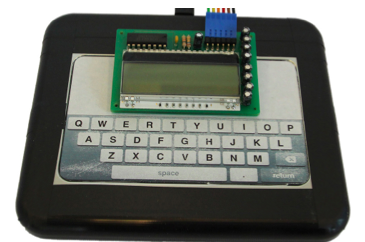
\includegraphics[width=0.6\linewidth]{forcetype}
	\begin{itemize}
		\item Modified Synaptics Forcepad
		\item Pressure mapped to Gaussian variance (no \ac{GP})
		\item System explained to users
		\item Users type phrases with and without forcetype
	\end{itemize}
\end{frame}

\begin{frame}
	\frametitle{ForceType: Results}
	\begin{multicols}{2}
		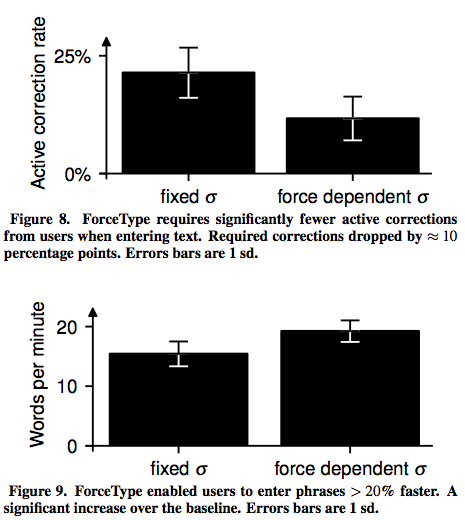
\includegraphics[width=\linewidth]{forcetype_results}
		\newpage
		\vfill
		\begin{itemize}
			\item Forcetype reduced number of corrections performed by users (top)
			\item Forcetype improved overall text entry rate
		\end{itemize}
		\vfill
	\end{multicols}
\end{frame}

\begin{frame}
	\frametitle{Conclusions}
		\begin{itemize}
			\item GP regression is key to the approach: we make no parametric assumptions (what would they be?)
			\item \ldots and get probabilistic predictions
			\item \ldots that can be fed to the \ac{SLM} -- (un)certainity is passed to the \ac{SLM}
			\item Performance is promising
			\item<2->Can also use pressure to provide explicit uncertainty control
			\item<3->More info:
			\begin{itemize}
				\item \url{http://www.youtube.com/watch?v=llQI5gV5l74}
				\item \url{http://pokristensson.com/pubs/WeirEtAlCHI2014.pdf}
				\item Acknowledgements: Daryl Weir, Per Ola Kristensson, Keith Vertanen, Henning Pohl
			\end{itemize}
		\end{itemize}
\end{frame}



\mode<all>
% Clinical ratings

\lecture{Application: Clinical Ratings}{Clinical}

\begin{frame}
	\frametitle{Clinicians disagree in AandE}
	\begin{itemize}
		\item Patients in \ac{AE} are continually monitored.
		\begin{itemize}
			\item Heart rate
			\item Blood pressure
			\item Temperature
			\item etc
		\end{itemize}
		\item<2-> Based on these hourly observations, clinicians (in a Glasgow hospital) give each patient an ordinal rating
		\begin{itemize}
			\item A (healthy(ish)), B, C, D, E, F (critical)
		\end{itemize}
		\item<3->These ratings are \emph{subjective}
		\begin{itemize}
			\item How do clinicians disagree? (variance? bias?)
		\end{itemize}
		\item<3->More details of this work in \href{http://dx.doi.org/10.1109/JBHI.2013.2252182}{Rogers et al 2013} and \href{http://dx.doi.org/10.1007/s11222-009-9125-z}{Rogers et al 2010}
	\end{itemize}
\end{frame}

\begin{frame}
	\frametitle{Data}
	\begin{itemize}
		\item $c = 1\ldots C$ clinicians.
		\item $p=1\ldots P$ patients.
		\item For patient $p$, we have $T_p$ observations at times $\mathbf{t}_p = [t_{p1},\ldots,t_{pT_p}]^T$.
		\item $y_{\tau c}^p$ is rating at $t_{p\tau}$ ($\{A,B,C,D,E\}$).
		\item The model:
		\begin{itemize}
			\item Patient health is modelled as a GP.
			\item Each clinician has their own offset and precision used to \emph{corrupt} the health function ($q$).
			\item $q$ is binned to produce rating.
		\end{itemize}
	\end{itemize}
\end{frame}

\begin{frame}
	\frametitle{Model}
	\begin{multicols}{2}
		\begin{figure}[tbh]
			\centering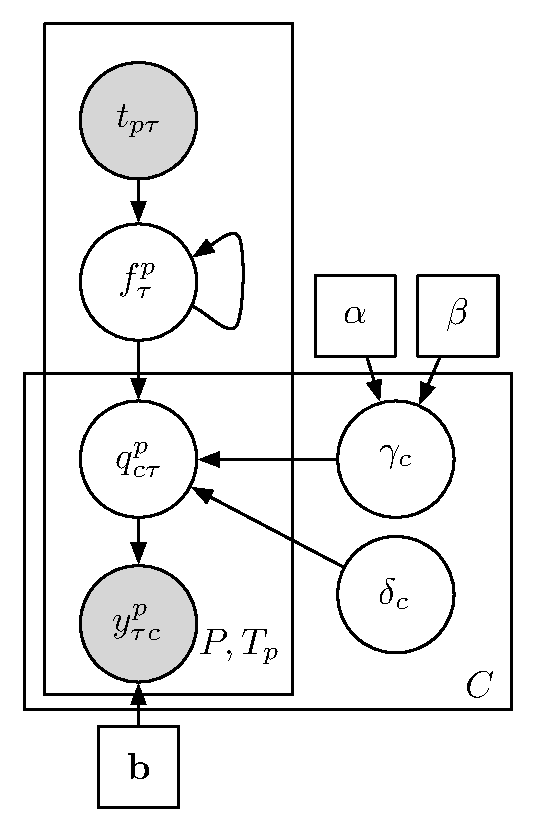
\includegraphics[width=0.9\linewidth]{ClinicalCartoon.pdf}
			\centering\caption{\label{fig:clincartoon}Plates diagram}
		\end{figure}
		\newpage
		\begin{eqnarray}
			\nonumber \blf^p &\sim & {\cal N}(\mathbf{0},\mathbf{C}^p)~~\mbox{[health]}\\
			\nonumber \delta_c &\sim & {\cal N}(0,1)~~\mbox{[offset]}\\
			\nonumber \gamma_c &\sim & {\cal G}(\alpha,\beta)~~\mbox{[precision]}\\
			\nonumber q_{c\tau}^p &\sim & {\cal N}(f_\tau^p + \delta_c,\gamma_c^{-1})\\
			\nonumber P(y_{\tau c}^p=k) &=& \delta(b_k < q_{c\tau}^p < b_{k+1})
		\end{eqnarray}
		Previously auxiliary variables were $z_n\sim {\cal N}(f_n,1)$. This model adds clinician-specific offsets and precisions: $q_{c\tau}^p \sim  {\cal N}(f_\tau^p + \delta_c,\gamma_c^{-1})$.
	\end{multicols}
\end{frame}

\begin{frame}
	\frametitle{Example data generation}
	\begin{figure}[tbh]
		\centering\includegraphics<1>[width=0.8\linewidth]{health.pdf}
		\centering\includegraphics<2>[width=0.8\linewidth]{health_corrupted.pdf}
		\centering\includegraphics<3>[width=0.8\linewidth]{health_corrupted_ratings.pdf}
		\centering\caption{\label{fig:health_example}Example of the generative process described by the model for three clinicans.}
	\end{figure}
\end{frame}

\begin{frame}
	\frametitle{Model inference}
	\begin{itemize}
		\item Gibbs sampling is straightforward
		\item We sample:
		\begin{itemize}
			\item The latent health function for each patient.
			\item The auxiliary variables.
			\item The offset and precision for each clinician.
		\end{itemize}
		\item<2->The offset and precision tell us how the clinicians disagree.
		\item<3->Identifiability: offset for one clinician fixed to 0.
	\end{itemize}
\end{frame}

\begin{frame}
	\frametitle{Results}
	\begin{figure}[tbh]
		\centering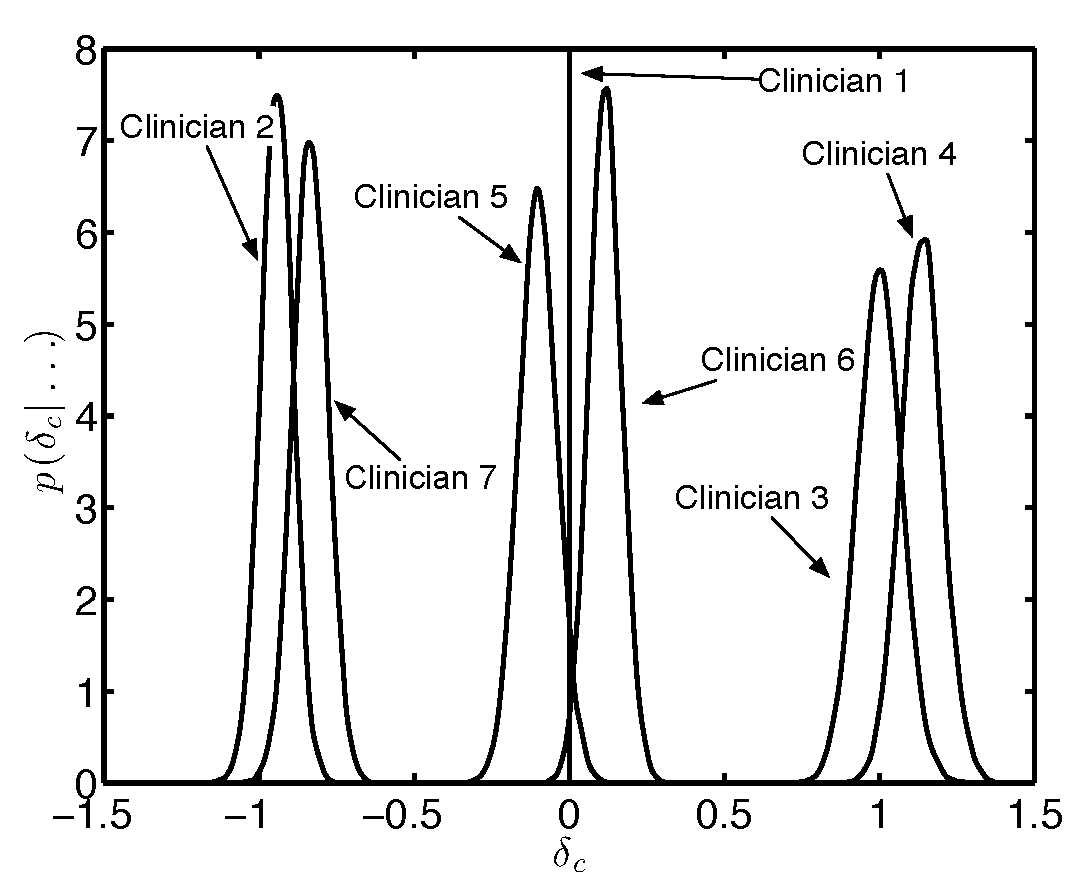
\includegraphics[width=0.8\linewidth]{offset.pdf}
		\centering\caption{\label{fig:offset}Marginal offset posteriors}
	\end{figure}
\end{frame}

\begin{frame}
	\frametitle{Results}
	\begin{figure}[tbh]
		\subfigure[Clinicians 2 and 4]{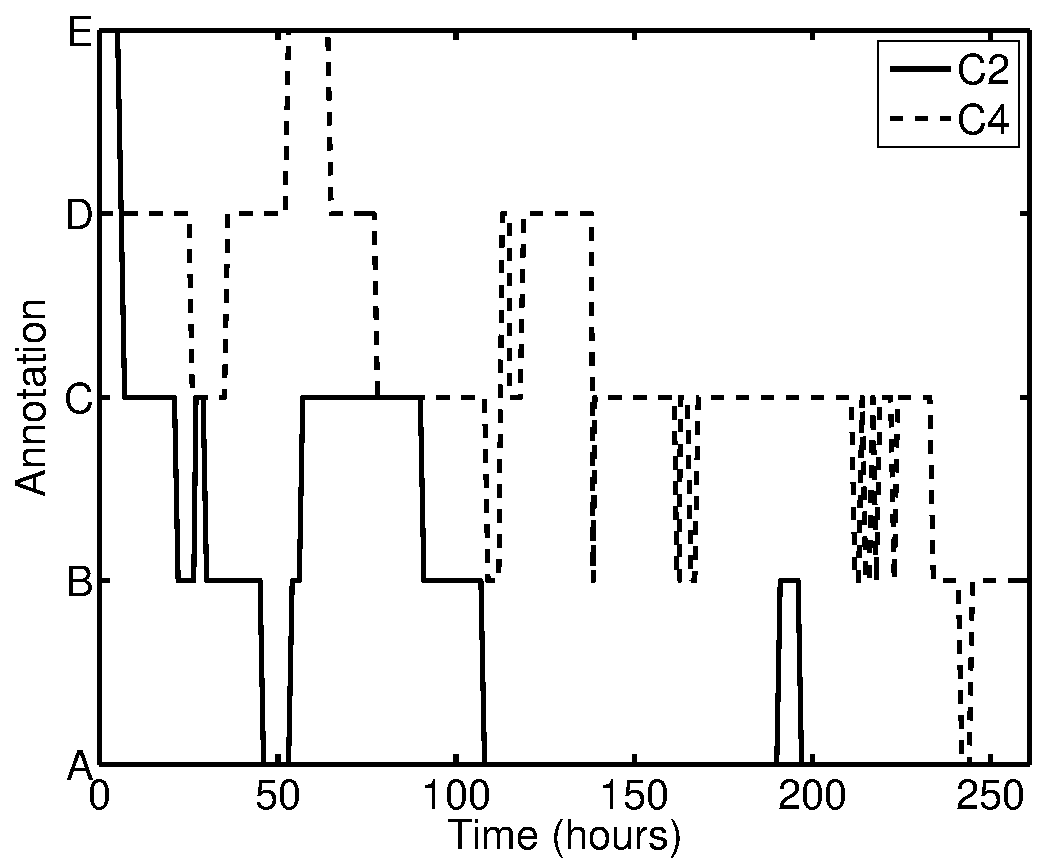
\includegraphics[width=0.45\linewidth]{P2_C24.pdf}}
		\subfigure[Clinicians 3 and 4]{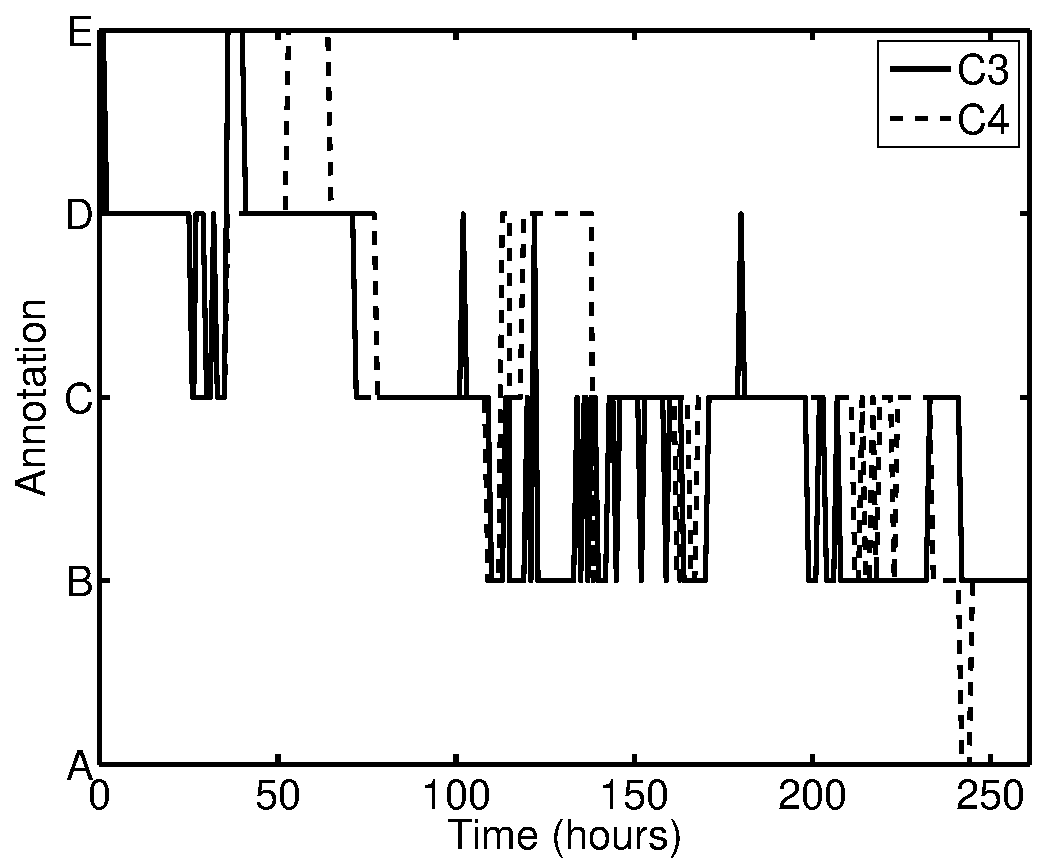
\includegraphics[width=0.45\linewidth]{P2_C34.pdf}}
		\centering\caption{\label{fig:actualratings}Inferred offsets make sense on inspection of the data.}
	\end{figure}
\end{frame}

\begin{frame}
	\frametitle{Results}
	\begin{figure}[tbh]
		\centering\includegraphics[width=0.8\linewidth]{precision_offset_box_17thApril.pdf}
		\centering\caption{\label{fig:clinicalprecision}Marginal precision posteriors. Clinicians 1, 4, and 8 appear to be the least consistent (wrt the majority)}
	\end{figure}
\end{frame}

\begin{frame}
	\frametitle{INSIGHT}
	\begin{itemize}
		\item After the initial annotation, clinicians went through INSIGHT procedure.
		\item The goal was to make ratings more consistent.
		\item If it succeeded, we should see a recuction in offset and increase in precision in the post-INSIGHT data.
	\end{itemize}
\end{frame}

\begin{frame}
	\frametitle{Post-INSIGHT results}
	\begin{figure}[tbh]
		\subfigure[Offsets]{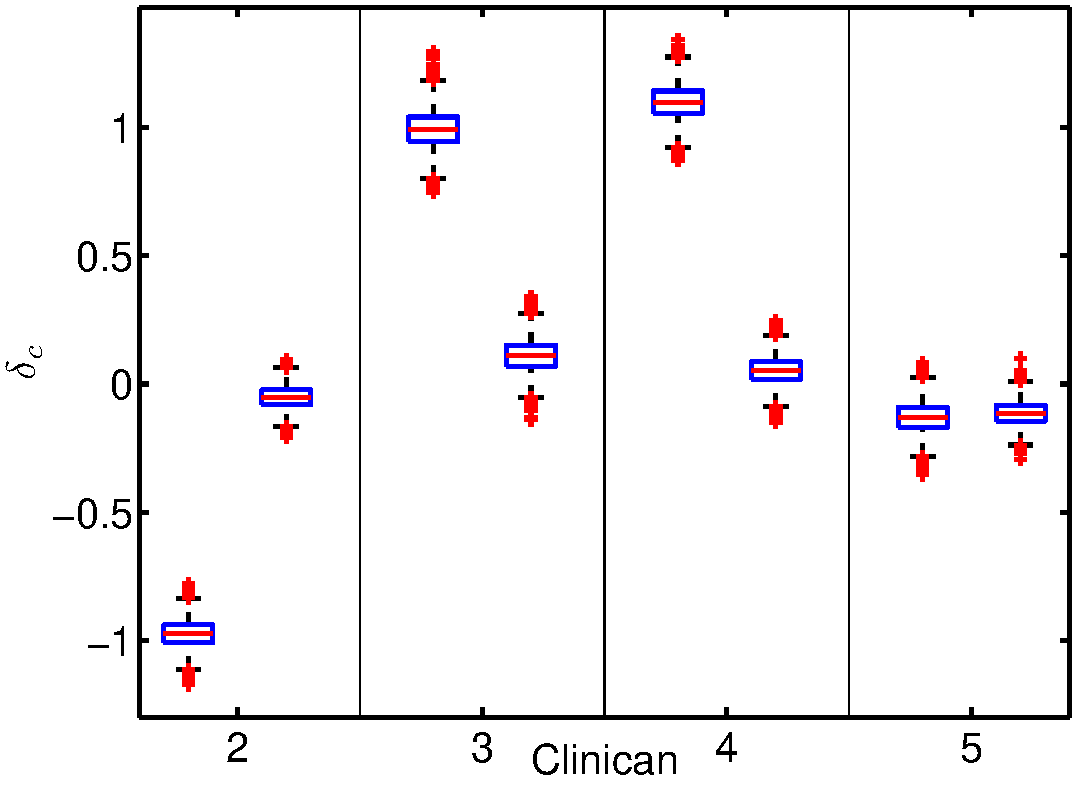
\includegraphics[width=.45\linewidth]{Offset_compare_before_after_17April.pdf}}\hfill
		\subfigure[Precisions]{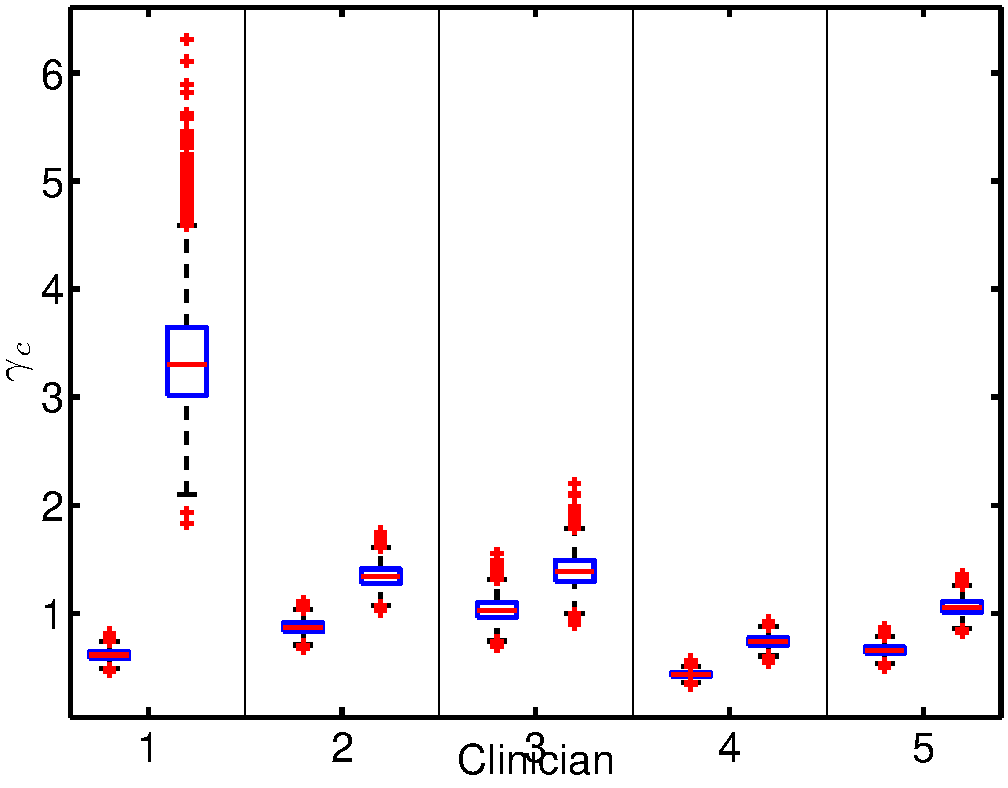
\includegraphics[width=.45\linewidth]{Precision_before_after_April19th.pdf}}
		\centering\caption{\label{fig:clinoffprec}Offsets and precision before and after INSIGHT. Offsets get closer to 0, whilst precision increase suggesting greater agreement amongsth clinicians.}
	\end{figure}
\end{frame}

\begin{frame}
	\frametitle{Inferring category boundaries}
	\begin{itemize}
		\item So far, it has been assumed that all categories are the same size (i.e. the elements of $\mathbf{b}$ are equally spaced).
		\item We can also infer these (with fixed end-points and $\delta_c=0$).
		\item Removes uniform prior assumption over categories.
	\begin{figure}[tbh]
		\subfigure[Before INSIGHT]{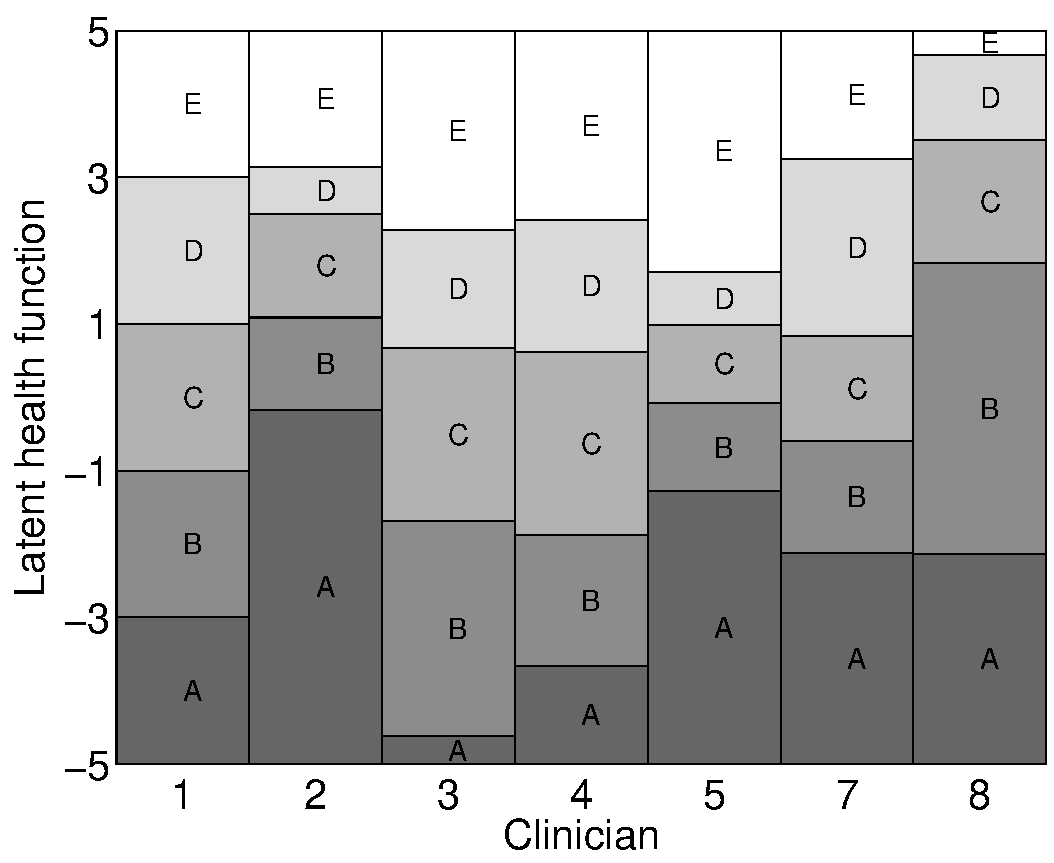
\includegraphics[width=0.45\linewidth]{start_thresh.pdf}}\hfill
		\subfigure[After INSIGHT]{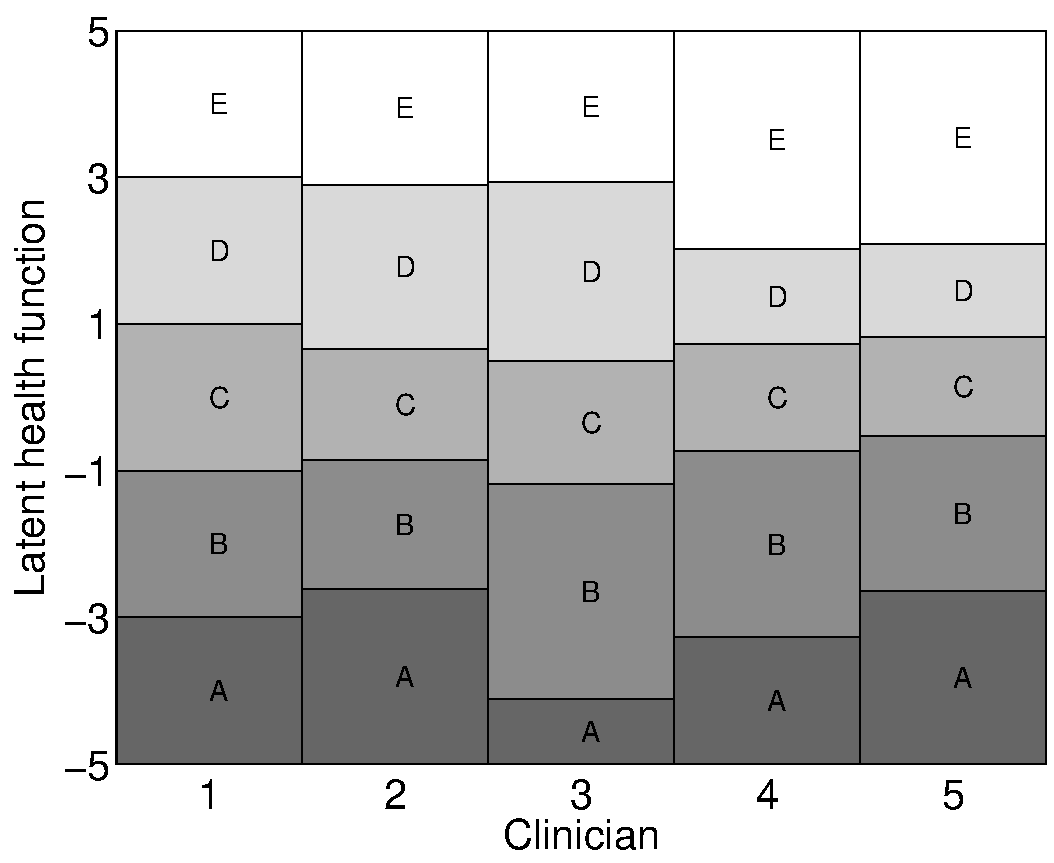
\includegraphics[width=0.45\linewidth]{end_thresh.pdf}}
		\centering\caption{\label{fig:clinicalcategories}Posterior mean cateogory boundaries.}
	\end{figure}
	\end{itemize}
\end{frame}

\begin{frame}
	\frametitle{Summary and Conclusions}
	\begin{itemize}
		\item Model allows us to:
		\begin{itemize}
			\item learn something about \emph{how} clinicians disagree and how they rate.
			\item assess the effectiveness of the INSIGHT procedure.
		\end{itemize}
		\item<2-> GP prior:
		\begin{itemize}
			\item Flexible
			\item Required no parametric assumptions about health function
			\item Hyper-parameter ($\gamma$) was inferred in the model (could be patient-specific)
		\end{itemize}
		\item<3-> Auxiliary Variable Trick:
		\begin{itemize}
			\item Not restricted to a standard Gaussian centered on the GP variable.
			\item Incorporated offset and precision without causing additional inference challenges.
		\end{itemize}
	\end{itemize}
\end{frame}
\end{document}